\chapter{Integração dos Dados}

O processo de integração de dados heterogêneos era frequentemente realizado pela abordagem virtual \cite{chawathe1994tsimmis} ou pela abordagem materializada \cite{Widom:1995:RPD:221270.221319}.
Na abordagem virtual os dados permanecem em fontes separadas e são integrados via consulta. Como pode-se observar na figura \ref{fig1}, a arquitetura dessa abordagem requer diferentes componentes. A aplicação envia consultas, que são interceptadas pelos mediadores, cuja função é direcionar para o tradutor correto, que por sua vez identifica a fonte de dados correta e efetivamente encontra a informação desejada. Caso a informação seja um dado bruto não estruturado, é requerido um classificador e extrator para a obtenção dos dados chave que representem a informação. O mediador é responsável ainda por unificar os resultados das consultas e trata-los se necessário. Os autores acreditam que pode haver um template para esses mediadores, de forma que os mesmos sejam gerados semiautomática ou automaticamente. Essa hipótese é exemplificada pelo gerador de mediadores e gerador de tradutores que devem ter esse papel.
A abordagem materializada por sua vez, possui além das fontes de dados, um empacotador que traduz as informações das fontes e um monitor que analisa a mudança nas fontes (novas fontes plugadas ou informações novas salvas em uma fonte). Em seguida os dados tratados são direcionados para o integrador que mescla os dados e os envia para o data warehouse. A arquitetura dessa abordagem pode ser analisada na \ref{fig2}. Data warehouses requerem que seus esquemas sejam definidos previamente, visto que os dados devem ser compreendidos antes da etapa de ETL (extração, transformação e carga) dos dados para o Data warehouse. As análises que são criadas unicamente no data warehouse tradicional dificultam o tratamento de dados que não estão em conformidade com um esquema bem definido, porque esses dados geralmente são descartados e perdidos.

\begin{figure}[!ht]
\centering
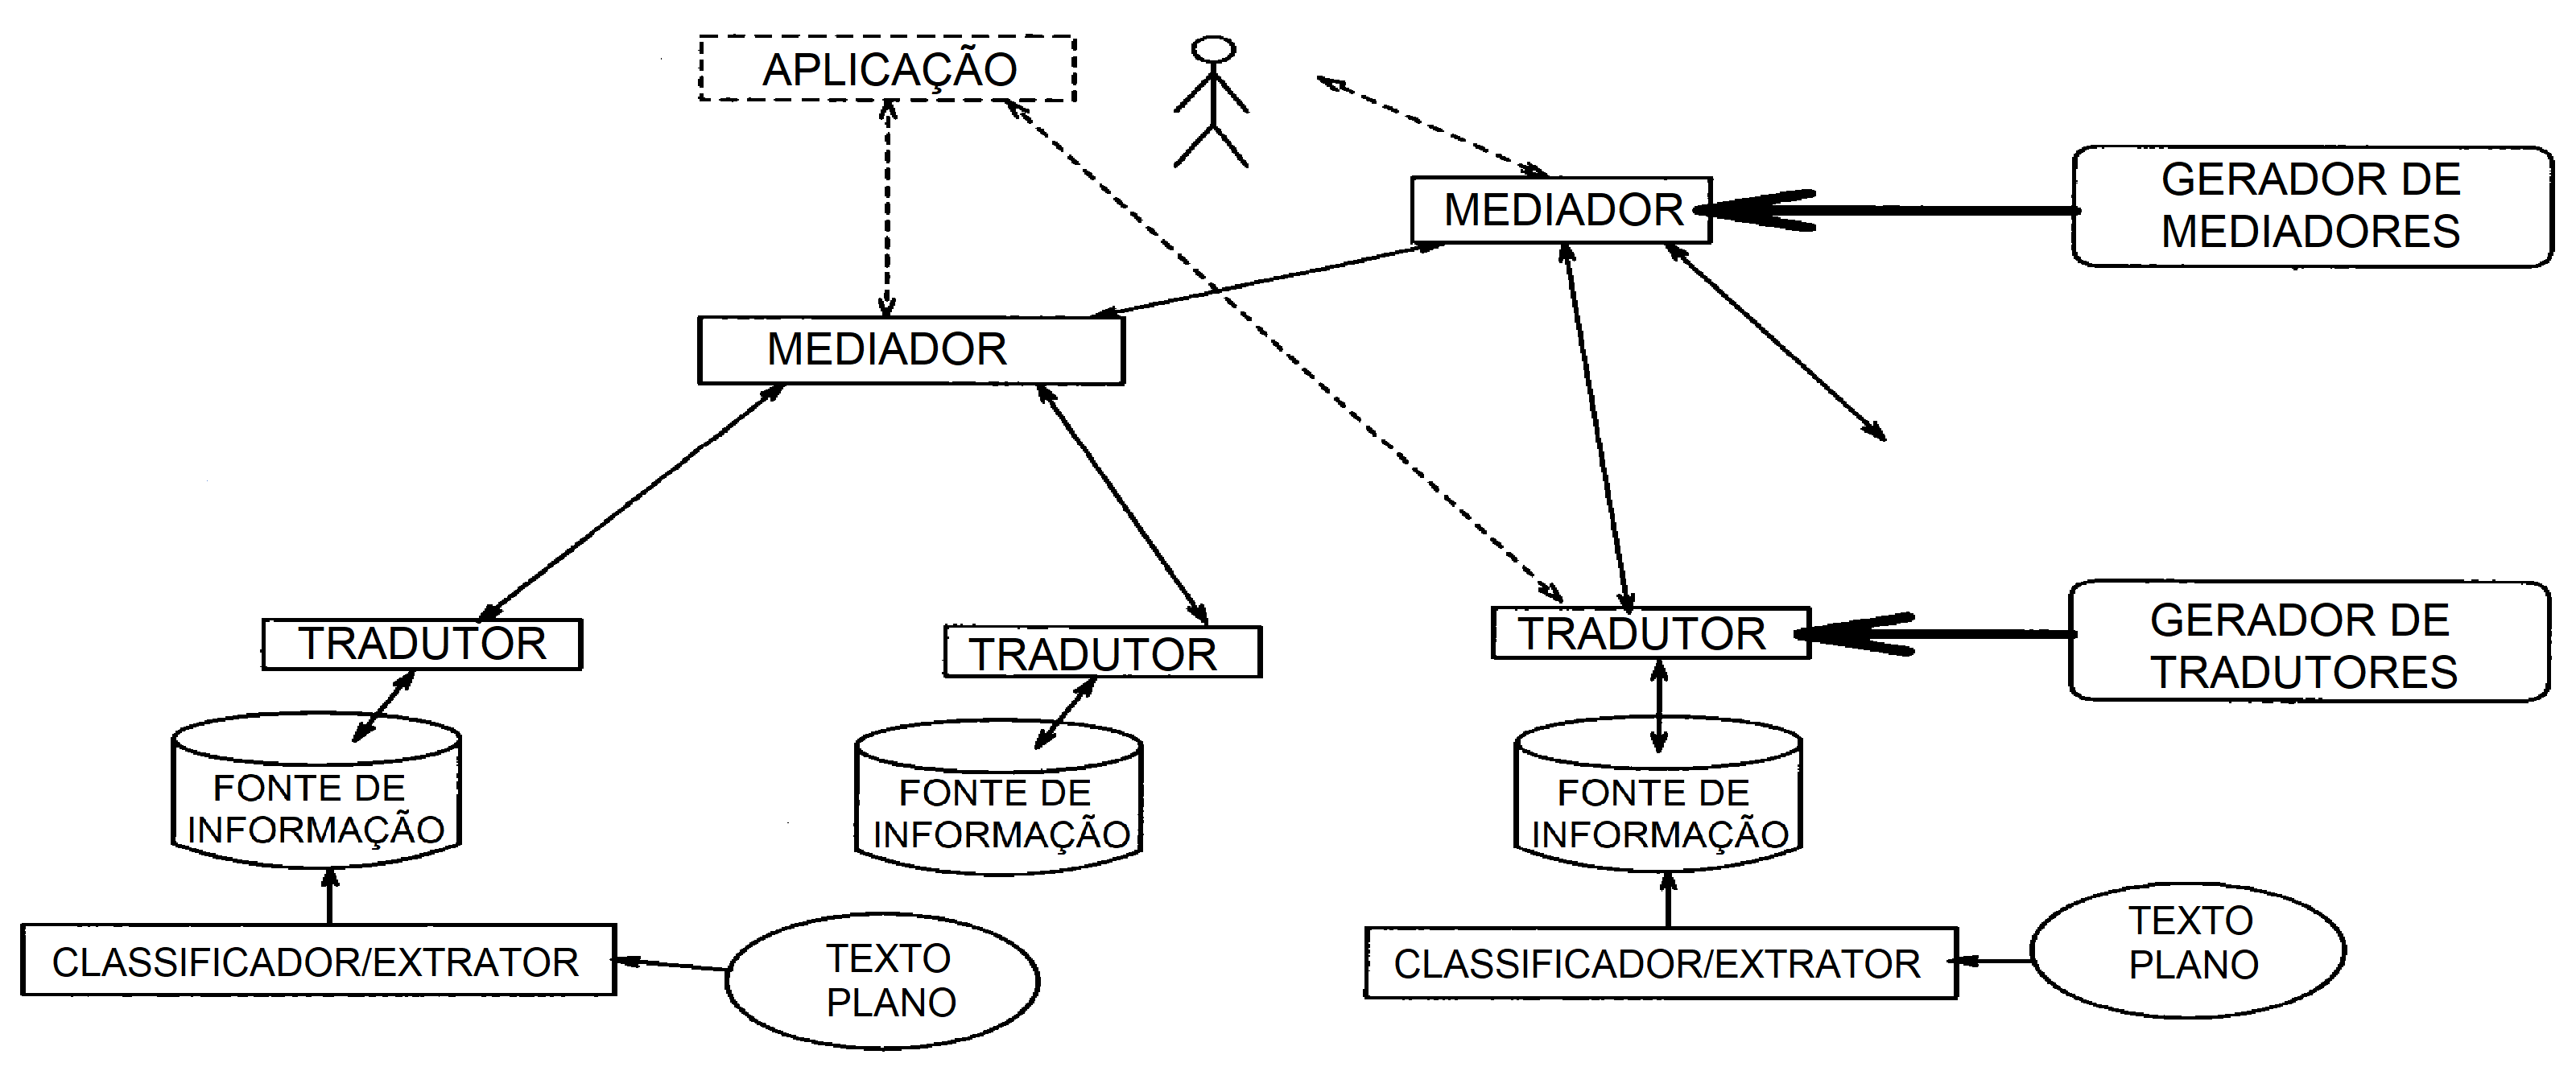
\includegraphics[width=0.3\linewidth]{figuras/TSIMMIS.png}
\caption{Abordagem virtual. Essa figura foi retirada e traduzida do artigo \cite{chawathe1994tsimmis}}
\label{fig1}
\end{figure}

\begin{figure}[!ht]
\centering
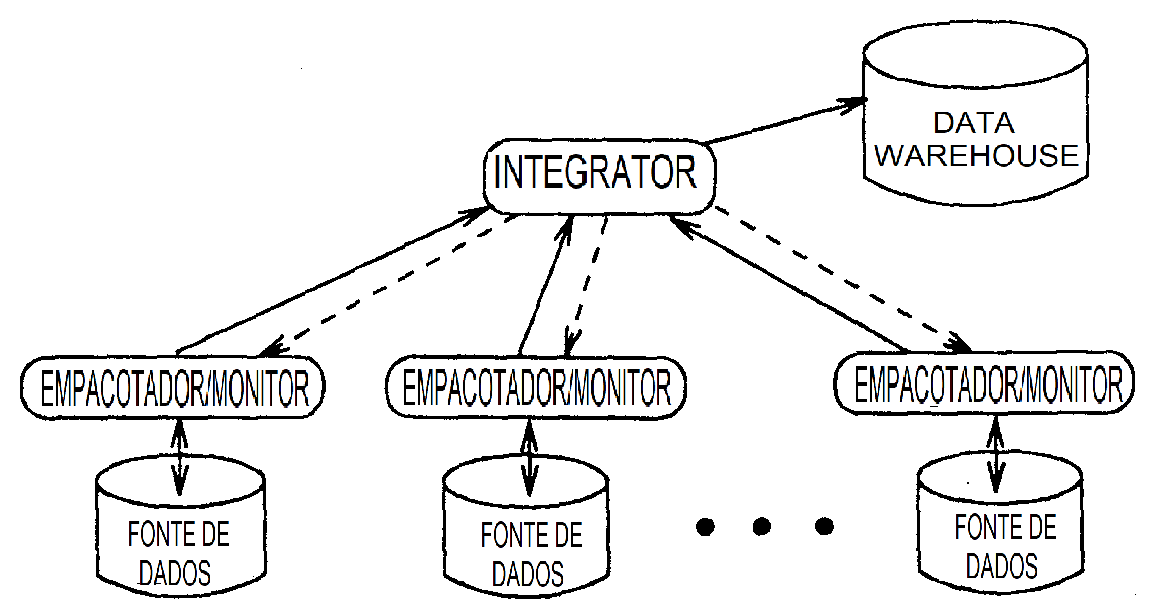
\includegraphics[width=0.3\linewidth]{figuras/DW.png}
\caption{Abordagem materializada com Data Warehouse. Essa figura foi retirada e traduzida do artigo \cite{Widom:1995:RPD:221270.221319}}
\label{fig2}
\end{figure}

No entanto, o volume de dados cresce vertiginosamente. Estima-se por exemplo que em 2020, a quantidade de dados não estruturados deverá ser em torno de 44 ZB \cite{turner2014digital}.
Dessa forma, os conjuntos de dados passaram a ter tal tamanho e estrutura que excedem as capacidades das ferramentas de programação tradicionais para coleta, armazenamento e processamento de dados em um tempo razoável e por motivos de força maior, excedem a capacidade de sua percepção por um humano \cite{miloslavskaya2014information}. Esses fatos invibializam as abordagens descritas anteriormente em um cenário de Big Data. Os critérios que determinam a diferença entre as abordagens tradicionais (virtual e materializada) de abordagens de Big Data são os 7V: Volume, Velocidade, Variedade, Veracidade, Variabilidade, Valor e Visibilidade.
Uma tecnologia recente de Big Data que tem mostrado bons resultados são os Data Lakes.
Um data lake é um repositório centralizado que permite armazenar todos os  dados estruturados, semiestruturados e não estruturados em qualquer escala. O armazenamento é feito no formato natural dos dados \cite{laskowski2016data}. Como exemplificado na figura \ref{fig3}, a preocupação é armazenar todos os dados, sem perda, para posterior exploração.

\begin{figure}[!ht]
\centering
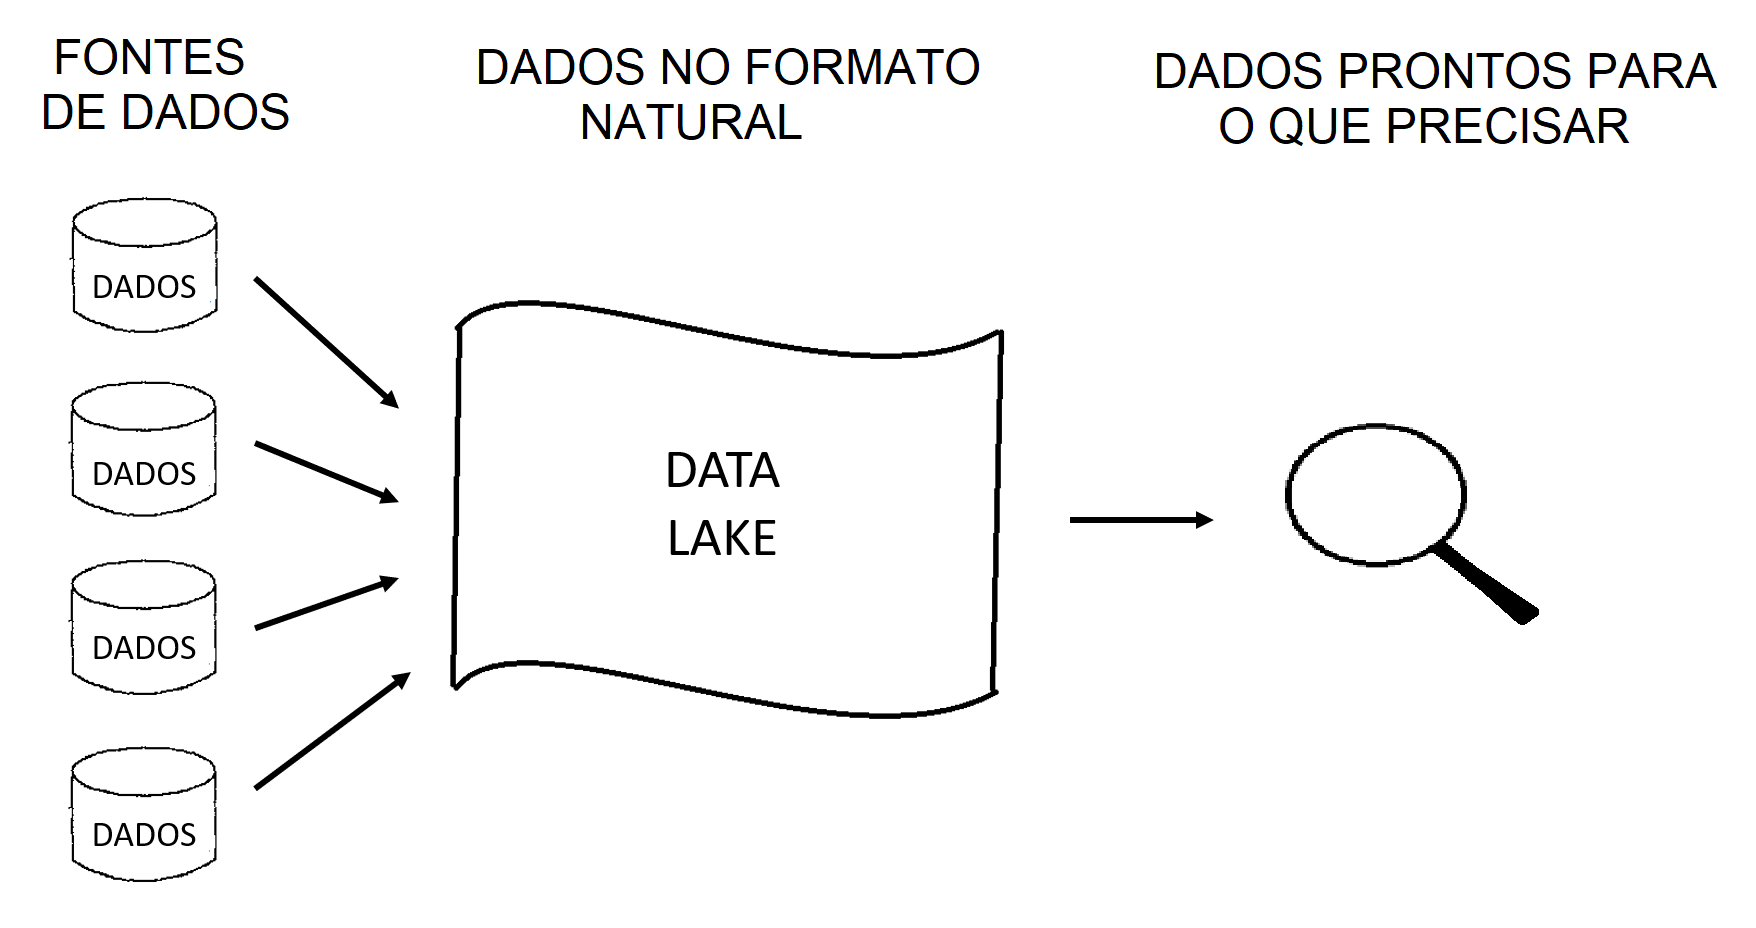
\includegraphics[width=0.3\linewidth]{figuras/DL.png}
\caption{Fluxo de um Data Lake}
\label{fig3}
\end{figure}

Um Data Lake possui as seguintes etapas:
• Injeção de dados: Os Data Lakes permitem que importar qualquer quantidade de dados que possa vir em tempo real. Os dados são coletados de várias fontes e movidos para o lago de dados em seu formato original. Esse processo permite que você dimensione para dados de qualquer tamanho, economizando tempo de definição de estruturas de dados, esquemas e transformações.
• Armazenar: depois de recuperados, os dados precisam ser armazenados em um formato durável e facilmente acessível.
• Processar e analisar: nessa etapa, os dados são transformados de brutos em informações acionáveis.
• Explorar e visualizar: a etapa final é a de conversão dos resultados da análise em um formato que facilite a extração de informações e o compartilhamento com os colegas.

Note que mover os dados de um armazenamento em Data WareHouse ou outras abordagens para a abordagem "armazenar tudo" de um  Data Lake é útil somente se ainda for possível extrair conhecimento de todos os dados.
Vale ressaltar que o principal desafio de uma arquitetura de Data Lake é que os dados brutos são armazenados sem supervisão do conteúdo.
existem várias ferramentas para data lake, como: Google Cloud Platform \ref{https://cloud.google.com/solutions/build-a-data-lake-on-gcp?hl=pt-br}{GCP}, \ref{https://aws.amazon.com/pt/big-data/datalakes-and-analytics/what-is-a-data-lake/?nc1=h_ls}{AWS}, \ref{https://azure.microsoft.com/pt-br/services/storage/data-lake-storage/}{Azure}.  Além de fornecer funcionalidades de Data Lake, estas ferramentas possibilitam o uso de mineração de dados, aprendizado de máquina e diversos outros recursos integrados.
Neste trabalho, utilizaremos o \ref{https://drill.apache.org/}{Apache Drill} para integrar os dados, nos valendo do conceito já apresentado de Data Lake.
O Apache Drill é um sistema distribuído gratuito e de código aberto, para análise ad-hoc interativa de conjuntos de dados de grande escala. Projetado para lidar com até
petabytes de dados espalhados por milhares de servidores, seu objetivo é responder a consultas ad-hoc em uma latência baixa.
A arquitetura do drill possui basicamente 3 camadas: usuário, processamento e fonte de dados.
A camada de usuário provê acesso aos dados por meio de interfaces (linha de comando, REST, API e drivers JDBC/ODBC). A camada de processamento permite plugar ou extender linguagens de consulta. Na camada dos dados, configura-se  o acesso as fontes de dado, local e/ou clusterizada. Essas fontes podem ser estruturadas, semiestruturadas ou não estruturadas. \cite{hausenblas2013apache}.